SDIPI signifie "Swiss Digital Identity and Privacy Institute", pouvant se traduire par "Institut Suisse de l'Identité Digitale et de la Vie Privée". Il s'agit d'une association crée pendant ce projet, dans le but initial de soutenir cette étude dans sa visibilité et dans sa légitimité. L'association aspire maintenant objectifs plus larges : Le but est de sensibiliser le public Suisse à la manière dont ses informations privées sont enregistrées, traitées, croisées et utilisées.

Ce projet marque donc la fondation de cette association. 

À l'occasion, un site web pour l'association a été crée. Celui-ci présente l'association y compris sa mission, ses membres, ses études et ses statuts.

\blockquote{We want to raise awareness about how private data are handled online, what kinds of footprints people leave, and how they can control how they appear to the web.}, présente le paragraphe "Our work" de la page d'accueil.

La figure~\ref{a-sdipi-logo} représente le logo de l'association. La figure~\ref{a-sdipi} montre un aperçu de la page d'accueil, accessible à l'adresse \url{https://www.sdipi.ch}.

\begin{figure}[h]
	\centering
	
\includegraphics[width=0.7\textwidth]{images/annexes/logo_sdipi}
	\caption{Logo officiel de l'association Swiss Digital Identity and Privacy Institute}
	\label{a-sdipi-logo}
\end{figure}

\begin{figure}[h]
	\centering
	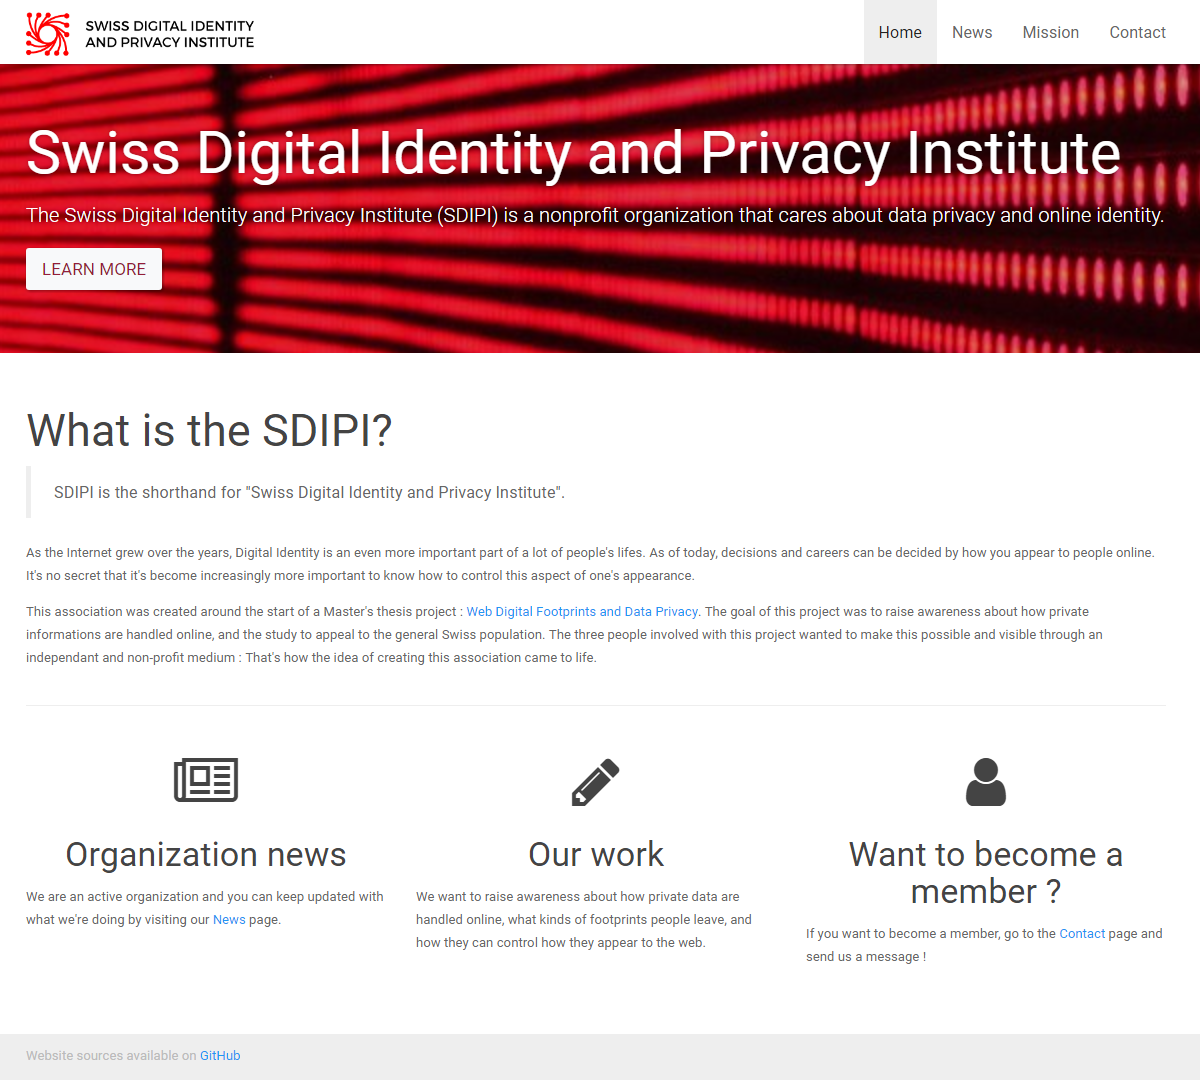
\includegraphics[width=1\textwidth]{images/design/sdipi_home}
	\caption{Page d'accueil du site web \url{https://sdipi.ch}.}
	\label{a-sdipi}
\end{figure}